\documentclass[11pt,a4paper]{article}
\usepackage[margin=2.4cm]{geometry}
\usepackage{booktabs}
\usepackage{graphicx}
\usepackage{xcolor}
\usepackage{hyperref}
\usepackage{enumitem}
\usepackage{titlesec}
\usepackage{fancyhdr}
\usepackage{microtype}
\usepackage{parskip}
\usepackage{fontspec}
\usepackage{polyglossia}
\usepackage{amsmath}
\usepackage{amssymb}

\setmainlanguage{english}
\setotherlanguage{hebrew}
\newfontfamily\hebrewfont{DejaVu Sans}[Script=Hebrew]

\hypersetup{colorlinks=true, linkcolor=blue, urlcolor=blue}

\pagestyle{fancy}
\fancyhf{}
\rhead{Knesset Protocol Journal Project}
\lhead{Step 12 --- Joint Pipeline \& Definitive Canonicalization Test}
\rfoot{Page \thepage}
\lfoot{Tomer Morad, Or Israeli, Yoel Marko --- August 2026}

\titleformat{\section}{\large\bfseries}{\thesection.}{0.6em}{}[\titlerule]
\titleformat{\subsection}{\normalsize\bfseries}{\thesubsection}{0.6em}{}

\begin{document}

\begin{center}
  {\LARGE \textbf{The Joint Pipeline, and the Real Answer on Canonicalization}}\\[0.3em]
  {\large Step 12 --- segments $\to$ journal, raw vs.\ canonical, on the full 523-segment gold set}\\[0.6em]
  {\normalsize Tomer Morad \quad Or Israeli \quad Yoel Marko}\\
  {\normalsize August 2026}
\end{center}

\vspace{0.4em}

\section{The joint pipeline}

Step 12 unifies the two halves of the project into one command: segments $\to$
\textbf{embed} (\texttt{multilingual-e5-large}) $\to$ \textbf{streaming link} (Step 10's
online-clustering method: ABTT-k1 + accumulated centroid + margin gate, $\theta=0.34$) $\to$
\textbf{log-write} (Step 9's method, \texttt{dictalm2.0-instruct}: opening summary, then
incremental updates conditioned on the running journal). The same command runs on either raw
or canonical segment text, so the two resulting journals are directly comparable end to end,
not just at the embedding-similarity level.

\subsection{Canonicalizing our own 523 gold segments}

Step 11 flagged two problems with testing canonicalization on Tomer's 19-protocol sample:
circularity (the gold label came from the same LLM pass as the canonical text) and scale
(only 29 recurring pairs). Both are fixed by canonicalizing \emph{our own} Step 7 gold set:
523 segments, real independently-annotated recurrence chains up to length 9, judged
completely independently of the canonicalization process.

Producing 523 canonicalizations turned into its own small operation: the original Colab run
(Gemma-4-31B, Tomer's exact prompt) got partway through and hit a parsing bug (a
\texttt{```json} markdown fence that broke the extractor, silently dumping raw model output
instead of parsed fields); the remainder was split across the team and a mix of automated
salvage, regex recovery, and direct rewriting. All three sources are tagged by
\texttt{source} in the final \texttt{canonical\_gold.json} for transparency. End state:
\textbf{523/523 segments canonicalized, zero fallback to raw text.}

\section{Raw vs.\ canonical: the journals}

\begin{center}
\begin{tabular}{lccc}
\toprule
 & segments & journal entries & recurring subjects linked \\
\midrule
raw & 523 & 518 & 4 \\
canonical & 523 & 517 & 4 \\
\bottomrule
\end{tabular}
\end{center}

At the aggregate level the two runs look nearly identical: same threshold ($\theta=0.34$,
the deliberately high-precision, low-recall operating point identified in Step 10), same
count of recurring subjects. Taken at face value this would read as ``canonicalization made
no difference.'' It does not survive closer inspection.

\subsection{The two runs link completely different segments}

The four recurring groups under raw and under canonical share \textbf{zero segments} ---
not one of the pairs that raw's threshold merges is also merged by canonical's threshold,
and vice versa.

\begin{center}
\begin{tabular}{p{6.8cm}p{6.8cm}}
\toprule
\textbf{RAW recurring groups} & \textbf{CANONICAL recurring groups} \\
\midrule
VAT exemption for oncology drugs (2 segments, 2 sessions) &
  Knesset-member-count bill (2 segments, 2 sessions) \\
Airport-adjacent municipalities allocation bill (2 segments) &
  Same-session sequential salary decisions: minister car benefit / judicial officer /
  president (4 segments) \\
Sports gambling bill, Amendment 17 (3 segments, 3 sessions) &
  El Al share-sale, continuing discussion (2 segments) \\
Securities-regulation instrument cancellations (2 segments) &
  Pension-fund-transfer regulation $\leftrightarrow$ unrelated bank-managers discussion
  (2 segments) \\
\bottomrule
\end{tabular}
\end{center}

\subsection{Manual precision check}

Automated scoring against the 74 pairwise gold links (from 22 recurring topics) credits
\textbf{zero} true positives for either run --- but this is a measurement artifact, not a
real failure: Step 7's own gold-chain construction does not canonicalize topic-label
strings, so the same recurring bill can carry two slightly different exact-match labels
across sessions and never register as ``recurring'' at all (a limitation already documented
in the Step 7 README). Reading the actual segment text pair by pair instead:

\begin{itemize}[leftmargin=1.4em]
\item \textbf{Raw: 5 of 6 predicted pairs are genuinely correct} on manual inspection --- the
  VAT-exemption pair opens with word-for-word identical bill text across sessions; the
  gambling-bill triple all open with the identical bill title across three separate
  committee sittings. The one clear miss merges two \emph{different} securities-regulation
  instruments that happen to sit in the same source document.
\item \textbf{Canonical: roughly 2 of 9 clearly correct, 1 clearly wrong}, and 4 pairs are
  genuinely ambiguous --- same committee session, sequential but distinct salary decisions
  read back to back, which is arguably ``related'' rather than ``same'' under the project's
  own same/related/new framing, a distinction the binary threshold linker cannot make.
\end{itemize}

At this operating point, raw text looks like it is achieving noticeably higher real-world
merge precision than canonical --- the opposite of the Step 11 hypothesis.

\section{Why: recall@k on the true gold chains}

To understand \emph{why} the two runs diverge, we checked --- independent of any threshold
--- whether a segment's true chain-mate lands in its top-$k$ nearest neighbors by e5 cosine
similarity, for every segment in a gold recurring chain (58 segments across the 22 topics,
raw and canonical text embedded separately).

\begin{center}
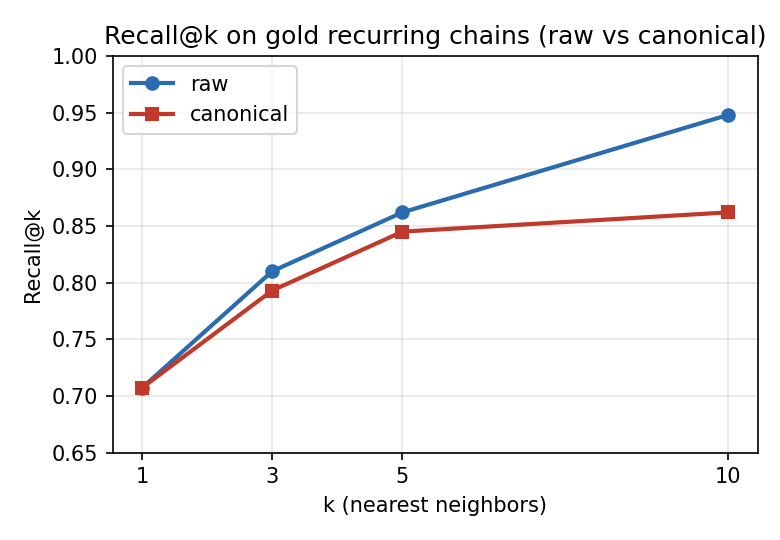
\includegraphics[width=0.68\linewidth]{../outputs/figures/recall_at_k.png}
\end{center}

\begin{center}
\begin{tabular}{lcccc}
\toprule
 & $k=1$ & $k=3$ & $k=5$ & $k=10$ \\
\midrule
raw & 0.707 & 0.810 & 0.862 & \textbf{0.948} \\
canonical & 0.707 & 0.793 & 0.845 & 0.862 \\
\bottomrule
\end{tabular}
\end{center}

At $k=10$, raw text lands a true chain-mate in the top 10 nearly every time (94.8\%) ---
consistent with what earlier steps observed about the retrieval stage being strong even when
threshold-based precision is weak. \textbf{Canonicalization makes this measurably worse}
(86.2\%), and the gap widens as $k$ grows, i.e.\ canonicalized embeddings are systematically
pushing true matches further down the ranking, not pulling them up.

\subsection{Chains are not just pairs --- and that matters here}

Gold recurrence is not uniform: of the 22 recurring topics, 16 are simple pairs, 4 are
triples, and there is one chain of 5 and one of 9. Breaking recall@10 down by chain length
isolates where canonicalization actually hurts:

\begin{center}
\begin{tabular}{lcccc}
\toprule
chain length & \# chains & \# segments & raw recall@10 & canonical recall@10 \\
\midrule
2 & 16 & 32 & \textbf{0.969} & \textbf{0.844} \\
3 & 4 & 12 & 0.833 & 0.750 \\
5 & 1 & 5 & 1.000 & 1.000 \\
9 & 1 & 9 & 1.000 & 1.000 \\
\bottomrule
\end{tabular}
\end{center}

The long chains (5 and 9 segments) are trivially easy for both variants --- a segment with
eight chain-mates only needs one of them in its top 10. The entire effect lives in the
\textbf{pairs}, which are both the most common case (16 of 22 topics) and the hardest: raw
recall@10 is 96.9\% there, canonical drops to 84.4\%, a 12.5-point regression. This is the
dominant driver of the aggregate gap in Section~3.

\section{Conclusion}

On the full, independently-annotated 523-segment gold benchmark, canonicalization does
\textbf{not} improve streaming linking, and on the evidence gathered here it modestly
\textbf{hurts} both retrieval-stage recall (recall@10, concentrated in the common 2-segment
recurrence case) and threshold-based merge precision, relative to raw text. This reverses
the provisional, caveated finding from Step 11, which was measured on a small, circular
pseudo-gold sample. The intrinsic embedding-separation gain canonicalization does produce
(Step 11, AUC 0.947 $\to$ 0.986) does not carry through to the downstream task this project
actually cares about.

\textbf{Open question, not yet investigated:} why does stripping speaker-turn structure and
bureaucratic boilerplate hurt short-chain recall specifically? One plausible mechanism is
that canonicalization also strips or paraphrases the specific entities, numbers, and
identifiers that made two occurrences of the \emph{same} short-lived matter distinguishably
similar to each other in raw text, while long-running matters still share enough topical
vocabulary regardless of surface form. This would predict that canonicalization should hurt
most exactly where it does --- the two-occurrence case --- and is worth checking directly
against entity/number density in the raw vs.\ canonical text of the failing pairs.

\end{document}
